\subsection{Map}
The purpose of the Map datatype is to represent 2D spatial data such as images of the Sun and 
inner heliosphere. It provides a wrapper around a data array and its associated
spatial coordinates and as well as meta data. The \texttt{Map} object provides 
convenience methods for many functions 
such as rotation and re-sampling as well as convenience visualisation 
functions, providing an easy to use as well as powerful interface. The \texttt{Map} object
also provides a convenient interface for loadings data from a variety of sources, typically
a FITS file as shown in Figure~\ref{code:aia_1}.

The architecture of the \texttt{Map} object consists of a template map called
\texttt{GenericMap} which is a subclass of \texttt{astropy.nddata.NDData}. \texttt{NDData} is a 
generic wrapper around a \texttt{ndarray} with a \texttt{.meta} attribute to store meta data.
As \texttt{NDData} is currently still in development, \texttt{GenericMap} does not make full
use of its capabilities but this inheritance structure provides 
for future integration of \texttt{astropy}. In order to provide instrument/
detector specific integration \textt{GenericMap} is subclassed on creation. 
Each subclass of \texttt{GenericMap} can register with the \texttt{Map} creation function (i.e. factory)
by implementing a method that returns \texttt{True} if matching meta data 
for that instrument or detector is found in the file header. The \texttt{Map} factory 
will then automatically return an instance of the specific \texttt{GenericMap} 
subclass. As of this version Sunpy has \texttt{Map} specialisations for the 
following instruments: 
\textit{YOHKOH/SXT},\textit{SOHO/EIT} and \textit{LASCO}, \textit{RHESSI}, 
\textit{STEREO/EUVI} and \textit{COR}, \textit{HINODE/XRT},
\textit{PROBA2/SWAP}, \textit{SDO/AIA} and \textit{HMI}, 
and \textit{IRIS} SJI frames. 

The \texttt{Map} object stores standard meta data retrieved in the header of 
the image file, via the \texttt{.meta} attribute and provides convenience 
properties for more standard meta data, \textit{i.e.} \texttt{.instrument}, 
\texttt{.wavelength} or \texttt{.coordinate\_system}. 
Listing \ref{code:aia_1} also demonstrates the quick plot functionality of 
\texttt{Map}, see Section \ref{subsec:Viz} for more discussion of plotting.

\begin{listing}[H]
\begin{minted}[bgcolor=bg]{pycon}
>>> import sunpy.map
>>> aiamap = sunpy.map.Map('aia_file.fits')
>>> aiamap.peek()
\end{minted}
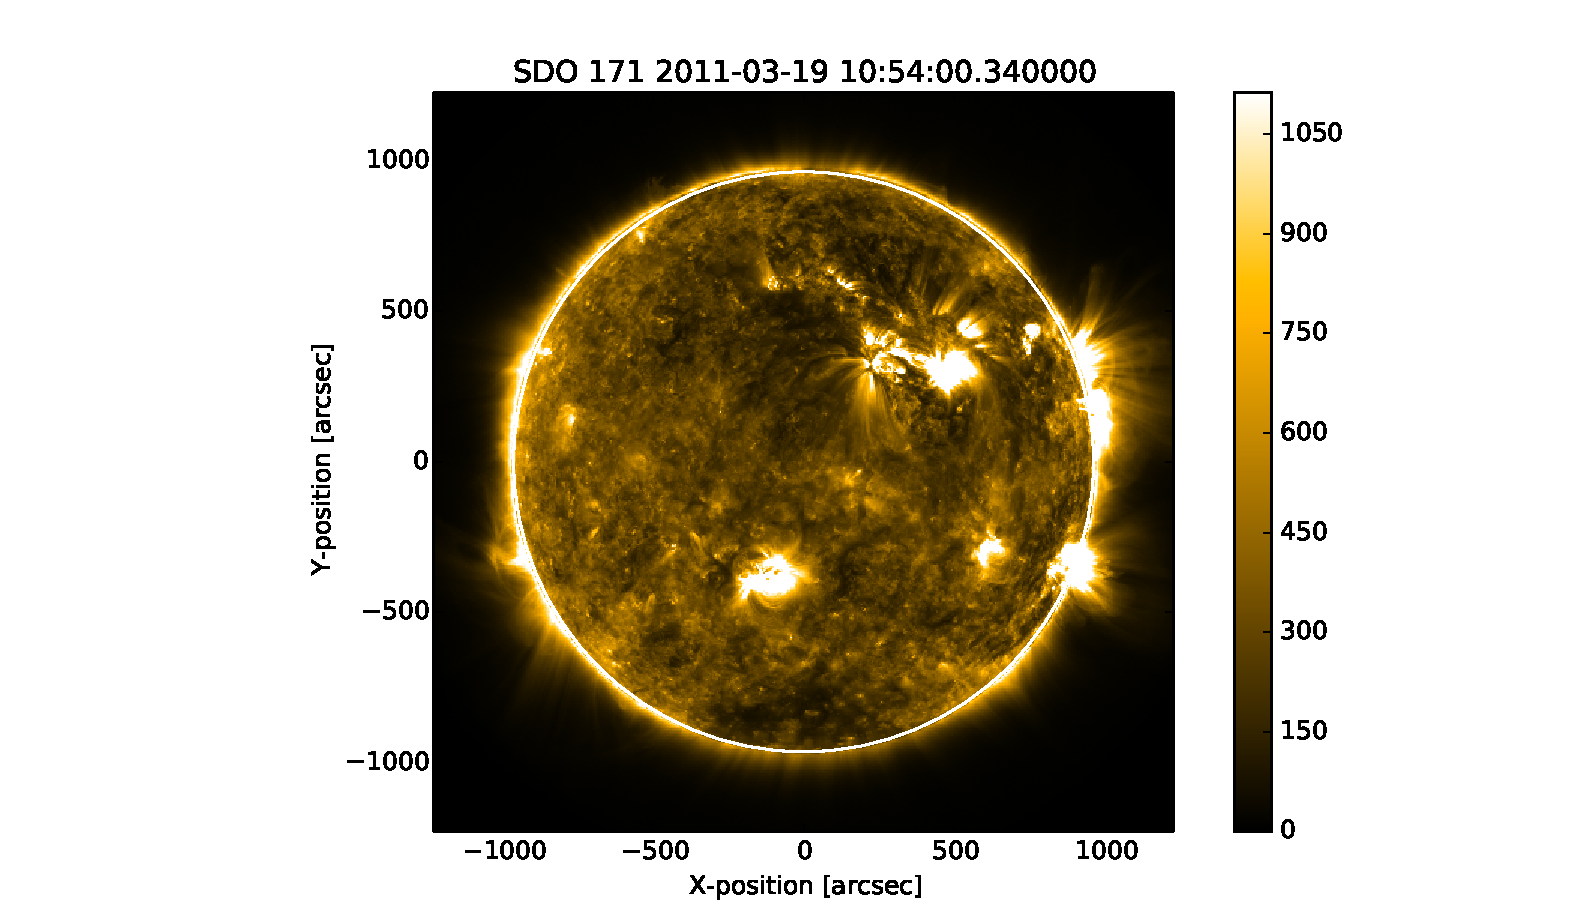
\includegraphics[width=0.8\columnwidth]{aia_map_example}
\caption{Demonstration of the \texttt{AIAMap} specialisation of 
\texttt{GenericMap}. The Map is created from an \textit{AIA} FITS file and the 
key meta data and array overview is printed. Then a quick view plot is created 
by using the \texttt{.peek()} method.}
\label{code:aia_1}
\end{listing}

As well as providing the base classes the map sub-package provides two 
collection classes, \texttt{CompositeMap} and \texttt{MapCube}, for 
temporally and spatially aligned data respectively.
\texttt{CompositeMap} provides methods for overlaying spatially aligned 
data, with support for visualisation of images and contour lines overlaid 
upon each other.
\texttt{MapCube} 
provides methods for animation of its series of \texttt{Map} objects. 
Figure~\ref{code:compmap_1} and \ref{code:mapcube_1} shows how to interact 
with these classes.
In addition, Figure~\ref{code:mapcube_2} demonstrates how the \texttt{MapCube} 
classes interacts with the \texttt{animation} module to save a video.

\begin{listing}[H]
\begin{minted}[bgcolor=bg]{python}
import matplotlib.pyplot as plt
import sunpy.map

#Create a composite map from two files
compmap = sunpy.map.Map('aia_1600_image.fits', 'RHESSI_image.fits', 
composite=True)

#Set the RHESSI image (index 1) to have contour levels and a red colour map.
compmap.set_levels(1,range(0,50,5),percent=True)
compmap.set_colors(1,'Reds_r')

#Plot the result and crop
ax = plt.subplot()
compmap.plot()
ax.axis([200,600,-600,-200])
\end{minted}
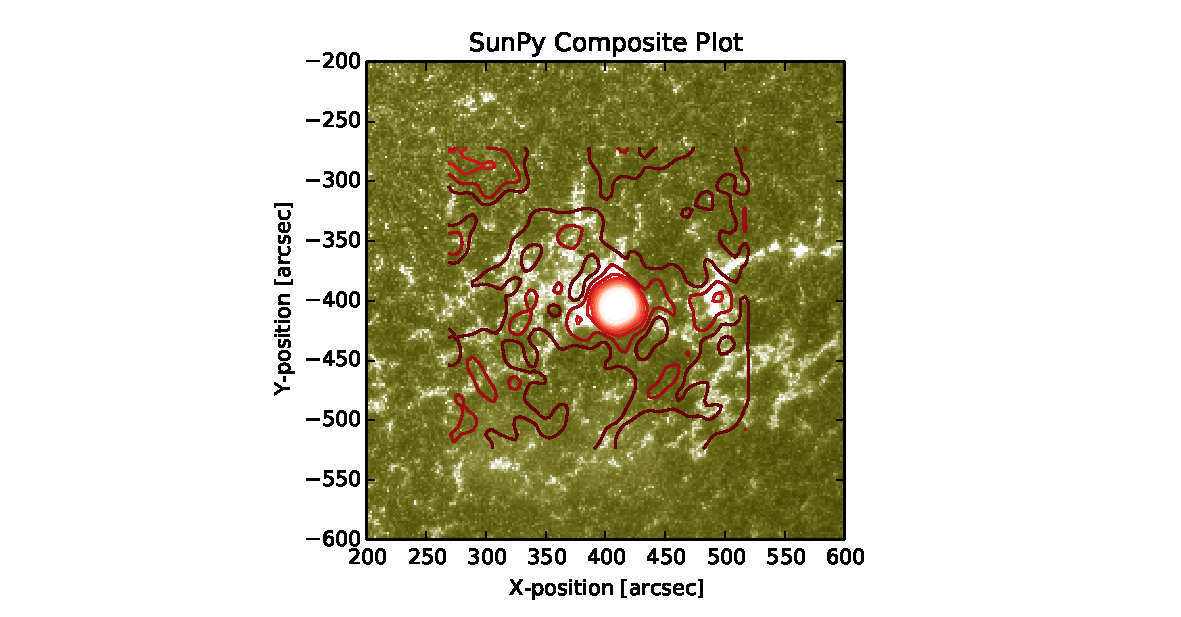
\includegraphics[width=0.8\columnwidth]{comp_map_example}
\caption{Example demonstrating a CompositeMap plot, using contours and how 
SunPy integrates with matplotlib's pyplot functional interface.}
\label{code:compmap_1}
\end{listing}

\begin{listing}[H]
\begin{minted}[bgcolor=bg]{python}
import sunpy.map

compmap = sunpy.map.Map('aia_lev1_171a_2014_01*fits', cube=True)
compmap.peek()
\end{minted}
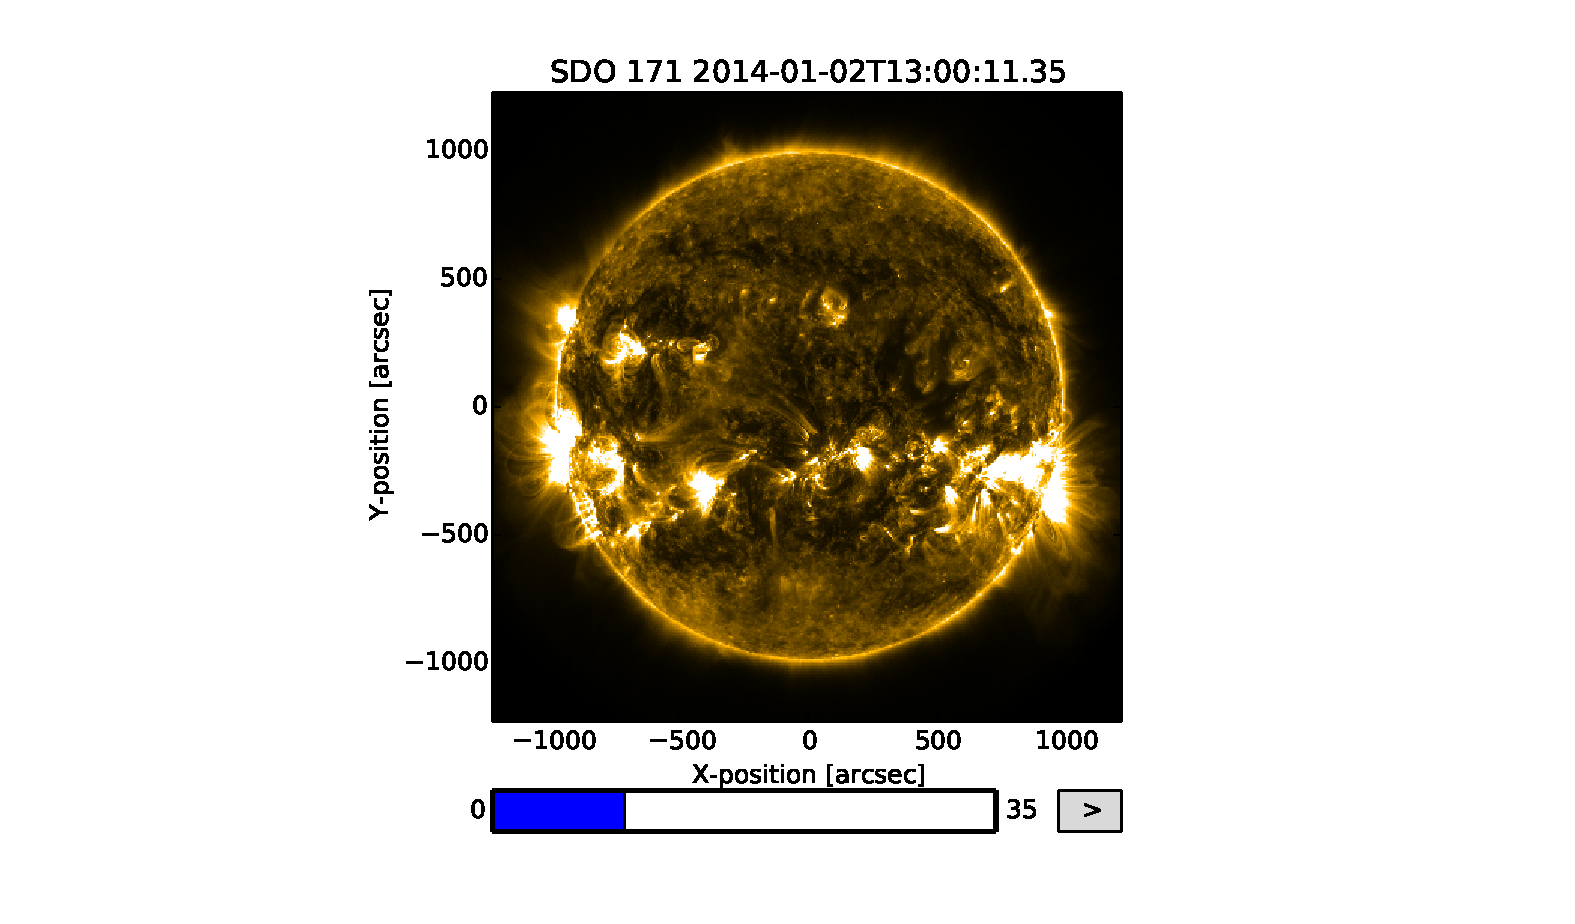
\includegraphics[width=0.8\columnwidth]{aia_cube_controls}
\caption{An example showing creation of a MapCube from a glob file search. The 
resultant plot makes use of matplotlib's interactive widgets to allow scrolling 
through the MapCube.}
\label{code:mapcube_1}
\end{listing}

\begin{listing}[h]
\begin{minted}[bgcolor=bg]{python}
import sunpy.map
from matplotlib import animation

mapc = sunpy.map.Map('aia_lev1_171a_2014_01*fits', cube=True)
anim = mapc.plot()
Writer = animation.writers['ffmpeg']
writer = Writer(fps=10, metadata=dict(artist='SunPy'), bitrate=1800)
anim.save('aia_cube.ogv')
\end{minted}
\caption{Example showing how to save a video animation from a MapCube, using 
matplotlib's animation framework.}
\label{code:mapcube_2}
\end{listing}
